\documentclass[a4paper,11pt]{article}

% -------------------------------------------------
% Packages
% -------------------------------------------------
\usepackage[utf8]{inputenc}
\usepackage[T1]{fontenc}
\usepackage[english]{babel}

\usepackage{graphicx}
\usepackage{float}
\usepackage{hyperref}
\usepackage{geometry}
\usepackage{xcolor}
\usepackage{setspace}
\usepackage{parskip}
\usepackage{microtype}

\geometry{margin=2.5cm}
\onehalfspacing

% -------------------------------------------------
% Title
% -------------------------------------------------
\title{
  \textbf{AR Tabletop Defense}\\[0.5em]
  \large An Augmented Reality Game using Unity and AR Foundation
}
\author{Cornelia Langsenlehner}
\date{\today}

\begin{document}
\maketitle

% -------------------------------------------------
\begin{abstract}
This project presents the development of a small-scale augmented reality game
for iOS using Unity and AR Foundation.
The goal was to design an intuitive and stable AR experience with a clear
gameplay loop while keeping the overall codebase compact and maintainable.
The resulting game demonstrates how simple mechanics, board-constrained enemy
movement, and camera-based interaction can be combined to create an engaging
tabletop AR experience.
\end{abstract}

\newpage
\tableofcontents
\newpage

% =================================================
\section{Introduction}

The goal of this project was the development of a simple but fully functional
augmented reality game for the iPhone.
The game was implemented using Unity and AR Foundation and was designed
specifically for mobile AR interaction.

During development, particular emphasis was placed on reliable plane detection,
intuitive player interaction, and a clear separation between game logic and
presentation.
In addition, the overall codebase was intentionally kept compact, with
approximately 735 lines of code.
This constraint encouraged a focused implementation and ensured that all
systems remained understandable and maintainable while still covering the
core aspects of an augmented reality game.

% =================================================
\section{Game Concept}

The developed game is called \textbf{AR Tabletop Defense}.
It is a simplified tower-defense-style game that is played on a virtual game
board placed on a real-world surface such as a table.

After the board has been placed, enemies spawn at the edges of the board and
move toward a central base.
The player must prevent the enemies from reaching the base by destroying them
beforehand.
Each enemy that reaches the base reduces the player’s remaining lives.
Once all lives are lost, the game ends.

Unlike traditional tower defense games, no defensive structures are placed.
Instead, the player acts as the sole defensive element through direct camera-
based interaction.

% =================================================
\section{Technical Implementation}

The project was developed using Unity 2022 LTS (2022.3.62f3) in combination with
AR Foundation and ARKit for iOS.
Version control was handled using Git and GitHub, allowing for structured and
traceable development.

\subsection{Technologies Used}

\begin{itemize}
  \item Unity 2022 LTS
  \item AR Foundation
  \item ARKit (iOS)
  \item C\#
  \item Git and GitHub
\end{itemize}

\subsection{AR Foundation Setup}

AR Foundation was used to detect horizontal planes in the user’s environment and
to place the virtual game board on a suitable surface.
The game relies on an AR Session and an XR Origin with an AR Camera.
Plane detection is restricted to horizontal surfaces to ensure a stable and
consistent gameplay experience.
Object placement is handled via raycasting against detected planes.

The spatial properties of the placed board are also used during gameplay.
Specifically, the physical size and position of the board are utilized to
constrain enemy movement paths.
This ensures that gameplay logic remains consistent with the real-world
placement of the augmented content.

% =================================================
\section{Gameplay Logic}

The game is structured around three main states: placing, playing, and game
over.
During the placing state, the player selects a suitable real-world surface and
places the game board.
Once placement is complete, the game transitions into the playing state, during
which enemies spawn and move toward the base.
When the player’s lives reach zero, the game enters the game-over state.

State management is handled centrally by a dedicated game manager component,
which controls transitions and updates the user interface accordingly.

\subsection{Enemy Behavior}

Enemies are spawned at predefined points along the edges of the game board.
Instead of moving directly toward the base along a straight line, enemies
follow procedurally generated paths that are constrained to the surface of the
placed AR board.

For each enemy, a set of random waypoints is generated within the bounds of the
board.
These bounds are derived from the renderer of the placed board object, ensuring
that all movement remains on the tabletop surface regardless of where or how
the board is positioned in the real world.
The final waypoint of each path is always the central base.

This approach introduces variation in enemy movement while preserving
predictable behavior.
It also strengthens the augmented reality aspect of the game, as enemy paths
are dynamically adapted to the physical placement and size of the board.
When an enemy reaches the base, it inflicts damage and is removed from the game.
Enemies can also be destroyed by the player before reaching their target.

% =================================================
\section{Interaction and Controls}

\subsection{Aiming System}

Player interaction is based on a camera-centered aiming system.
Instead of rendering a visible laser beam, a fixed crosshair is displayed in the
center of the screen.
The player aims by physically moving the device.

A raycast is continuously emitted in the forward direction of the camera.
If this ray intersects an enemy, the enemy is destroyed.
This interaction method feels natural in an augmented reality context and avoids
visual artifacts that can occur with rendered laser beams.

\subsection{User Interface}

The user interface provides the player with essential information, including the
current score, remaining lives, and status messages indicating the current game
state.
The interface was implemented using TextMeshPro to ensure clear and readable text
on mobile devices.

% =================================================
\section{Code Structure}

The project is organized into modular scripts, each responsible for a clearly
defined task.

\begin{itemize}
  \item \texttt{ARPlaceOnPlane.cs} handles the placement of the game board.
  \item \texttt{GameManager.cs} manages game states, score, and lives.
  \item \texttt{Spawner.cs} controls enemy spawning and difficulty progression.
  \item \texttt{Enemy.cs} manages enemy lifecycle, damage, and scoring.
  \item \texttt{EnemyPathFollower.cs} generates and follows randomized movement paths constrained to the AR board bounds.
  \item \texttt{CameraRayWeapon.cs} implements the camera-based aiming system.
  \item \texttt{HUD.cs} manages the user interface.
\end{itemize}

This modular structure improves readability and simplifies future extensions.

% =================================================
\section{Version Control}

The project is versioned using Git and hosted on GitHub.
Unity-generated directories such as the Library folder, build outputs, and other
temporary files are excluded from version control.
This approach keeps the repository lightweight and avoids platform-specific
issues.

% =================================================
\section{Screenshots}

\begin{figure}[H]
  \centering
  \begin{minipage}{0.32\textwidth}
    \centering
    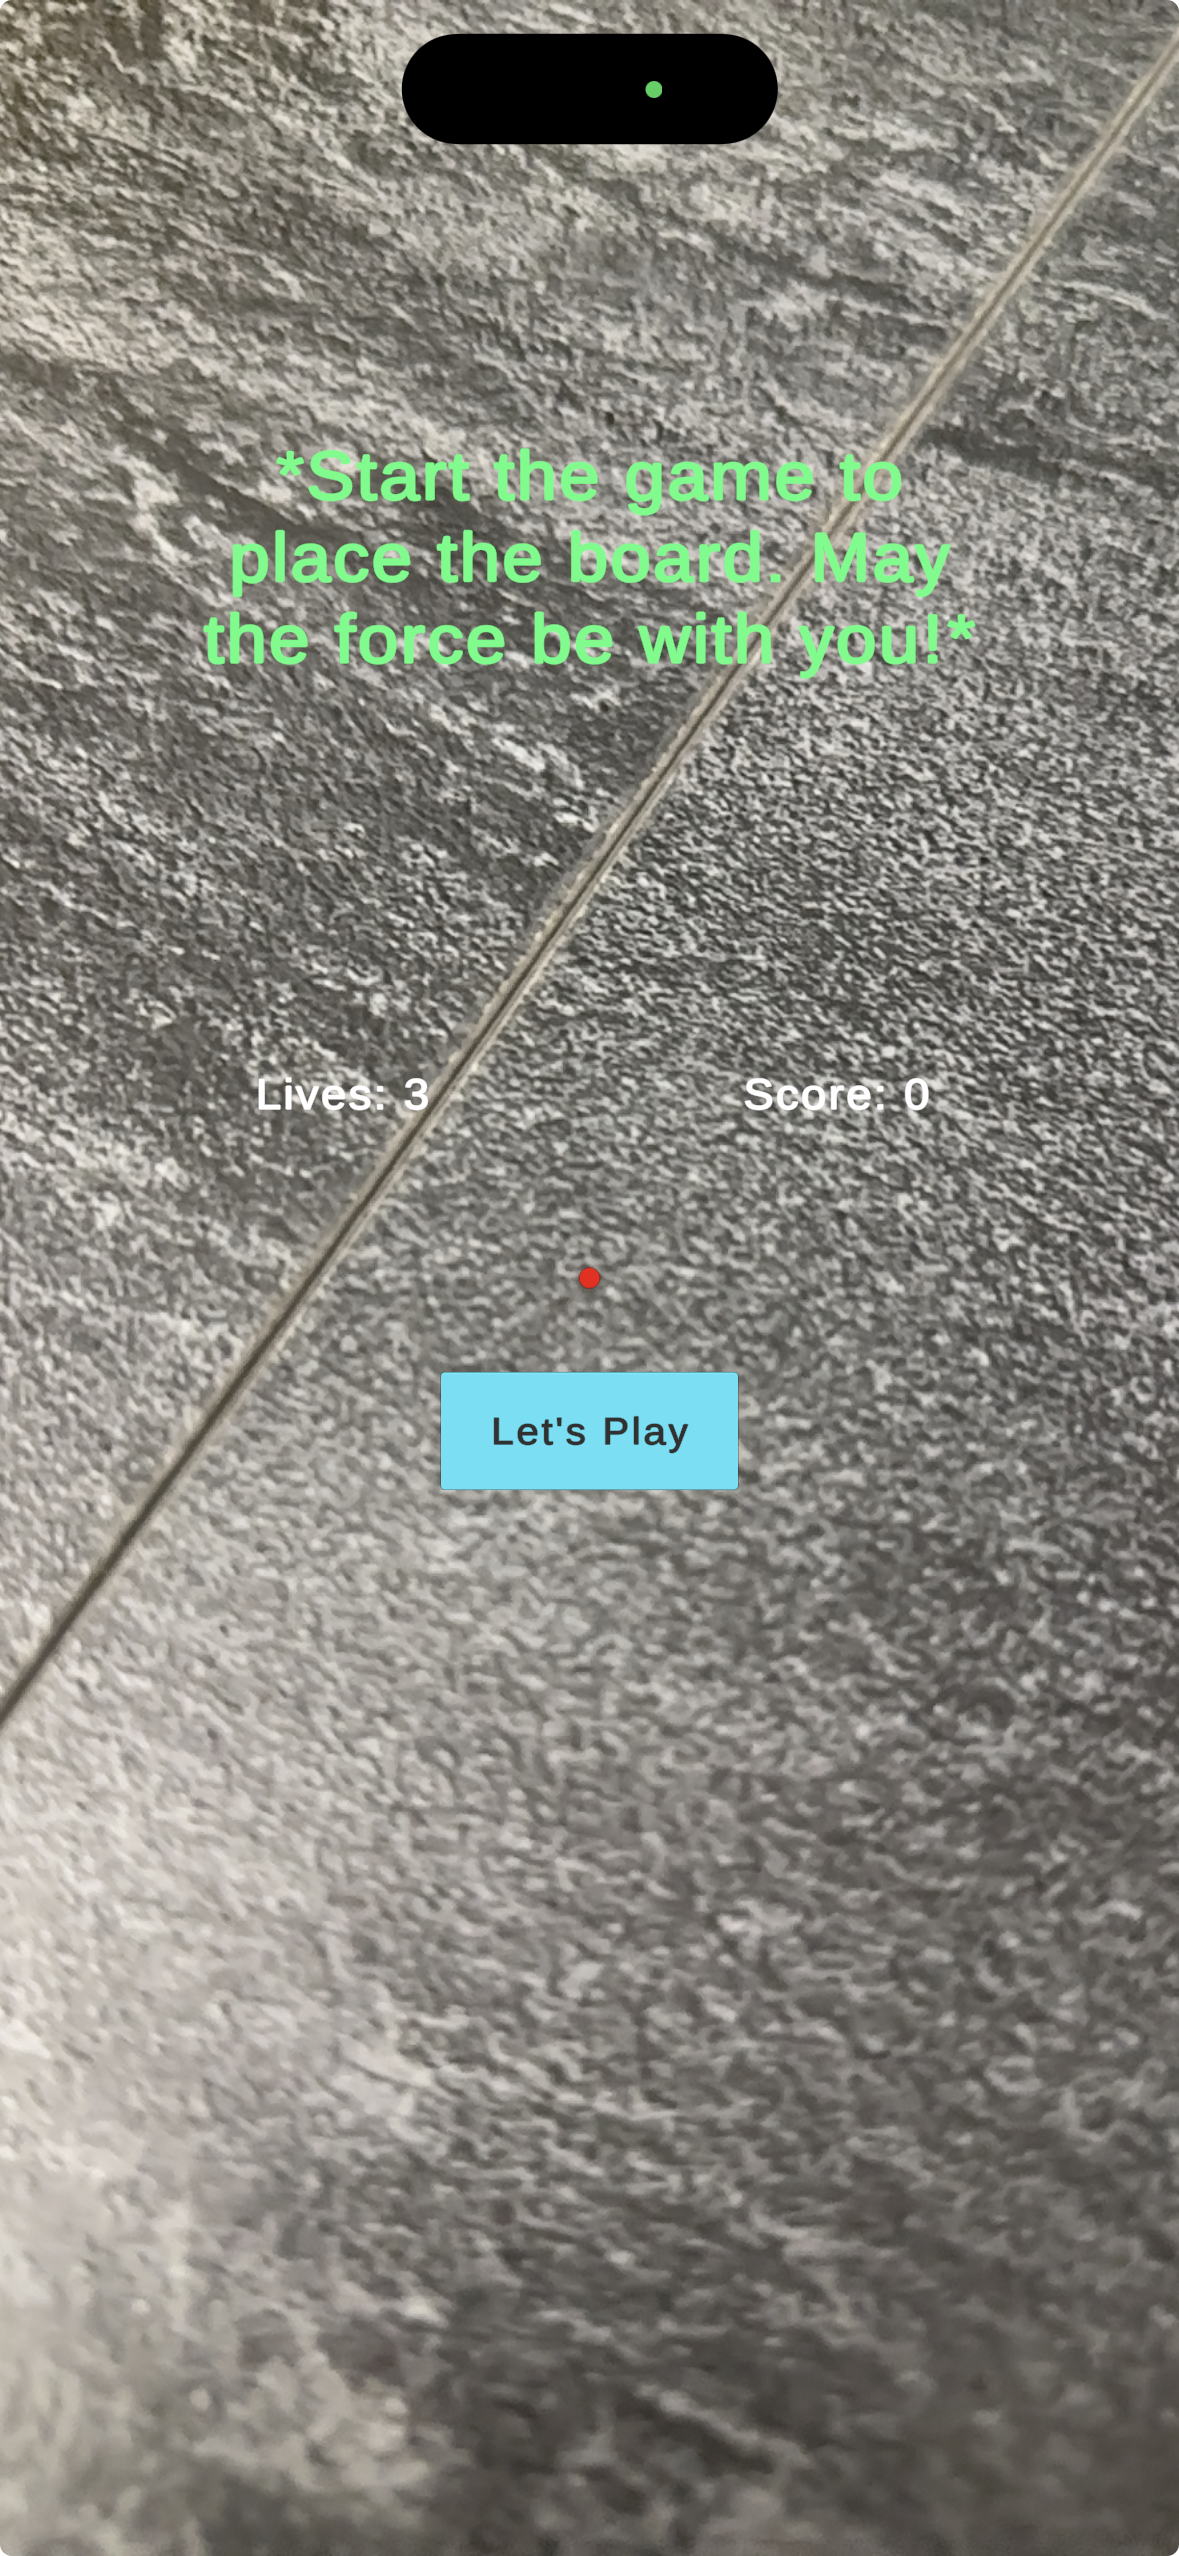
\includegraphics[width=\linewidth]{screenshot_placement.png}
    \caption*{(a) Board placement}
  \end{minipage}\hfill
  \begin{minipage}{0.32\textwidth}
    \centering
    \includegraphics[width=\linewidth]{screenshot_gameplay.png}
    \caption*{(b) Gameplay}
  \end{minipage}\hfill
  \begin{minipage}{0.32\textwidth}
    \centering
    \includegraphics[width=\linewidth]{screenshot_gameover.png}
    \caption*{(c) Game over}
  \end{minipage}

  \caption{Screenshots of the AR Tabletop Defense game showing placement, gameplay, and the game-over state.}
\end{figure}

% =================================================
\section{Conclusion}

This project demonstrates the successful development of a functional augmented
reality game for iOS using Unity and AR Foundation.
By combining simple mechanics with camera-based interaction and board-constrained
enemy movement, a stable and intuitive AR experience was achieved.

The modular structure and clear separation of responsibilities provide a solid
foundation for future extensions, such as additional enemy types, wave-based
difficulty progression, or further visual and audio polish.

\end{document}
